\documentclass[letterpaper, twoside, 12pt]{book}
\usepackage{packet}


\begin{document}

\setcounter{chapter}{1}

\chapter{Part 1: Sections 13.3-13.4}

\setcounter{chapter}{13}
\setcounter{section}{2}

\section{Arc Length and Curvature}

          \begin{problem}
            Let $\vect{r}(t)=\<6t, t^3, 3t^2\>$. Use the lengths of
            the line segments
            connecting $\vect{r}(0)$, $\vect{r}(1)$, $\vect{r}(2)$,
            and $\vect{r}(3)$ to approximate the length of the curve
            from $t=0$ to $t=3$.
          \end{problem}

          \begin{solution}

          \end{solution}

\begin{definition}
Let $\harpvec{r}(t) = \<f(t),g(t),h(t)\>$ be a vector function.
Then the \textbf{arclength} or \textbf{length} of the curve given by
$\harpvec{r}(t)$ from $t=a$ to $t=b$ is
\[
  L
    =
  \int_a^b
  \left|
    \lim_{\Delta{t}\to0}
    \frac{\vect{r}(t+\Delta{t})-\vect{r}(t)}{\Delta{t}}
  \right|
  \dvar{t}
  =
  \int_a^b |\vect{r}'(t)| \dvar{t}
\]
\end{definition}

          \begin{problem}
            Find the length of the curve given by
            $\vect{r}(t)=\<6t, t^3, 3t^2\>$
            from $t=0$ to $t=3$.
            (Hint: $9t^4+36t^2+36$ is a perfect square polynomial.)
          \end{problem}

          \begin{solution}

          \end{solution}

\begin{definition}
Let $s(t)$ be the \textbf{arclength function/parameter} representing the
length of a curve from the point given by
$\harpvec{r}(0)$ to the point given by $\harpvec{r}(t)$.
(Assume $s(t)<0$ for $t<0$.)
\end{definition}

\begin{theorem}
The arclength function $s(t)$ is given by the definite integral
\[
  s(t)
    =
  \int_0^t |\vect{r}'(\tau)| \dvar{\tau}
\]
\end{theorem}

\begin{theorem}
The derivative of the arclength function gives the lengths of
the tangent vectors given by the derivative of the position function:
\[
  \frac{ds}{dt} = \left|\frac{d\vect{r}}{dt}\right|
\]
\end{theorem}

          \begin{problem}
            Compute $s(t)$ for $\vect{r}(t)=\<6t, t^3, 3t^2\>$,
            and use it to find the arclength parameter corresponding
            to $t=-2$.
          \end{problem}

          \begin{solution}

          \end{solution}

          \begin{problem}
            Find the length of an arc of the circular helix with
            vector equation
            $\vect{r}(t) = \<\cos(t),\sin(t),t\>$
            from $(1,0,0)$ to $(1,0,2\pi)$.
          \end{problem}

\begin{definition}
  The \textbf{unit tangent vector} $\vect{T}$ to a curve $\vect{r}$ is the
  direction of the derivative $\vect{r}'(t)=\frac{d\vect{r}}{dt}$.
\end{definition}

\begin{theorem}
  \[
    \vect{T} = \frac{d\vect{r}/dt}{|d\vect{r}/dt|} = \frac{d\vect{r}}{ds}
  \]
\end{theorem}

          \begin{problem}
            Find the unit tangent vector to the curve given by
            $\vect{r}(t)=\<3t^2,2t\>$ at the point where $t=-3$.
          \end{problem}

          \begin{solution}

          \end{solution}

\begin{definition}
  The \textbf{curvature} $\kappa$ of a curve $C$ at a given point is
  the magnitude of the rate of change of $\vect{T}$ with respect to
  arclength $s$.
\end{definition}

\begin{theorem}
  \[
    \kappa
      =
    \left|
    \frac{d\vect{T}}{ds}
    \right|
      =
    \left|
    \frac{1}{ds/dt}
    \frac{d\vect{T}}{dt}
    \right|
      =
    \frac{1}{|d\vect{r}/dt|}
    \left|
      \frac{d\vect{T}}{dt}
    \right|
  \]
\end{theorem}

\begin{theorem}
  An alternate formula for curvature is given by
  \[
    \kappa =
    \frac{|\vect{r}'(t)\times\vect{r}''(t)|}{|\vect{r}'(t)|^3}
  \]
\end{theorem}

          \begin{problem}
            Prove that the helix given by the vector equation
            $\vect{r}(t) = \<\cos(t),\sin(t),t\>$
            has constant curvature.
          \end{problem}

          \begin{solution}

          \end{solution}

          \begin{problem}
            (OPTIONAL)
            Prove that the alternate formula for curvature is
            accurate by showing
            \[
              \frac{1}{|d\vect{r}/dt|}
              \left|
                \frac{d\vect{T}}{dt}
              \right|
                =
              \frac{|\vect{r}'\times\vect{r}''|}{|\vect{r}'|^3}
            \]
            (Some of the solution has been provided.)
          \end{problem}

          \begin{solution}
            Begin by observing that
            $
              \vect{r}'
                =
              \left|\frac{d\vect{r}}{dt}\right|\vect{T}
                =
              \frac{ds}{dt}\vect{T}
            $, and by the product rule it follows that
            $
              \vect{r}''
                =
              \frac{d^2s}{dt^2}\vect{T} + \frac{ds}{dt}\vect{T}'
            $.

            (...)

            % (Continue this argument by taking the cross-product of
            % $\vect{r}'$ and $\vect{r}''$, simplifying by using the fact that
            % $\vect{v}\times\vect{v}=\vect{0}$, then taking its magnitude
            % and simplifying using the fact that $|\vect{T}|=1$ and
            % $\vect{T},\vect{T}'$ are perpendicular (why?).
            % You should end up with
            % $\left(\frac{ds}{dt}\right)^2\left|\vect{T}'\right|$, which can
            % be used with $\frac{ds}{dt}=|\vect{r}'|$ to finish the proof.)
          \end{solution}

\begin{definition}
  The \textbf{unit normal vector} $\vect{N}$ to a curve $\vect{r}$ is the
  direction of the derivative of the unit tangent vector
  $\vect{T}'(t)=\frac{d\vect{T}}{dt}$.
  (By definition, this vector points into the direction of the curve.)
\end{definition}

\begin{theorem}
  \[
    \vect{N} = \frac{\vect{T}'}{|\vect{T}'|}
  \]
\end{theorem}

          \begin{problem}
            Prove that $\vect{N}$ actually is normal to the curve by
            using a theorem from a previous section. (Hint: $|\vect{T}|=1$.)
          \end{problem}

          \begin{solution}

          \end{solution}

          \begin{problem}
            Plot the curve given by $\vect{r}(t)=\<\cos(2t),\sin(2t)\>$,
            along with $\vect{T},\vect{N}$ at the point where
            $t=\frac{\pi}{2}$.
          \end{problem}

          \begin{problem}
            Give formuals for $\vect{T},\vect{N}$ in terms of $t$ for
            the vector function
            \[\vect{r}(t) = \< \sqrt{2}\sin t,2\cos t,\sqrt{2}\sin t \>\]
          \end{problem}

          \begin{solution}

          \end{solution}

\begin{definition}
  The \textbf{binormal vector} $\harpvec{B}$ is the direction
  normal to both $\harpvec{T}$ and $\harpvec{N}$ according to
  the right-hand rule.
\end{definition}

\begin{theorem}
  \[
    \vect{B}=\vect{T}\times\vect{N}
  \]
\end{theorem}

          \begin{problem}
            Prove that $\vect{T}\times\vect{N}$ is a unit vector.
          \end{problem}

          \begin{solution}

          \end{solution}

          \begin{problem}
          Given the following information about $\vect{r}(t)$ at a point,
          evaluate the binormal vector $\vect{B}$ and curvature
          $\kappa$ at that same point:
            \[\frac{d\vect{r}}{dt}=\<-3,0,3\sqrt{3}\>\]
            \[\frac{d\vect{T}}{dt}=\<-\sqrt{3},0,-1\>\]
            \[\vect{T}=\<-\frac{1}{2},0,\frac{\sqrt{3}}{2}\>\]
            \[\vect{N}=\<-\frac{\sqrt{3}}{2},0,-\frac{1}{2}\>\]
          \end{problem}

          \begin{solution}

          \end{solution}

\begin{definition}
  A \textbf{right-handed frame} is a group of three unit vectors which
  are all normal to one another and satisfy the right hand rule.
\end{definition}

\begin{example}
  $\veci,\vecj,\veck$ and $\vect T,\vect N,\vect B$ are examples
  of right-handed frames.
\end{example}

\begin{center}
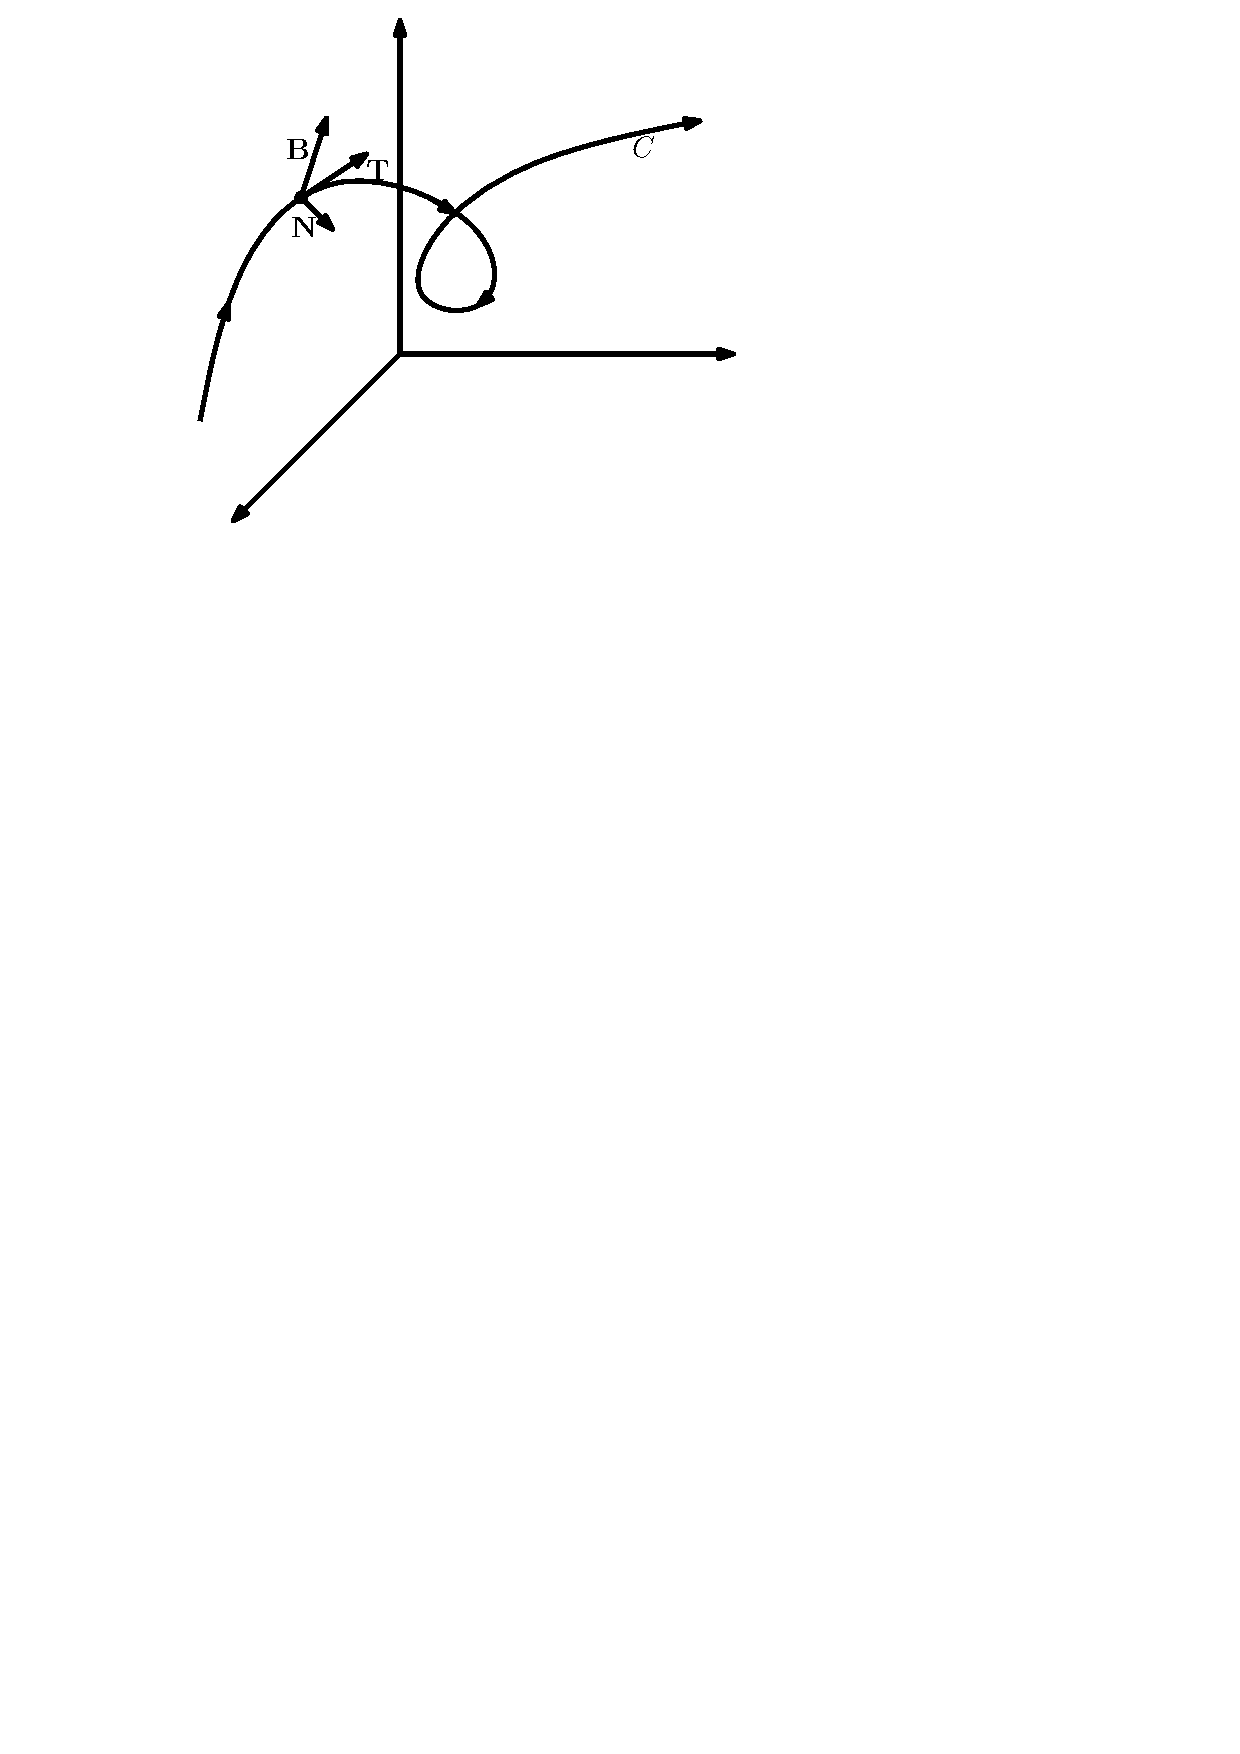
\includegraphics[width=0.5\linewidth]{assets/tnb.pdf}
\end{center}

\begin{theorem}
  Any vector is a linear combination of the vectors in a right-handed frame.
\end{theorem}

% \begin{suggestedHW}
%   Section $13.3: 1-6, 17-25, 49,50.$
% \end{suggestedHW}

\section{Motion in Space, Velocity, and Acceleration}

\begin{definition}
The \textbf{velocity} $\vect{v}(t)$ of a particle at time $t$ on a position
function $\vect{r}(t)$ is its rate of change with respect to $t$.
\end{definition}

\begin{definition}
The \textbf{speed} $|\vect{v}(t)|$ of a particle at time $t$ on a position
function $\vect{r}(t)$ is the magnitude of its velocity.
\end{definition}

\begin{definition}
The \textbf{direction} $\vect{T}(t)$ of a particle at time $t$ on a position
function $\vect{r}(t)$ is the direction of its velocity.
\end{definition}

\begin{definition}
The \textbf{acceleration} $\vect{a}(t)$ of a particle at time $t$ on a position
function $\vect{r}(t)$ is the rate of change of its velocity with respect to $t$.
\end{definition}

\begin{theorem}
\[
  \vect{v}(t)=\vect{r}'(t)
\]
\[
  |\vect{v}(t)|=|\vect{r}'(t)|=\frac{ds}{dt}
\]
\[
  \vect{T}(t) = \frac{\vect v}{|\vect v|}
\]
\[
  \vect{a}(t)=\vect{v}'(t)=\vect{r}''(t)
\]
\end{theorem}

\begin{problem}
  Given a position function $\harpvec{r}(t) = \<t^3,t^2\>$ find its velocity,
  speed, and acceleration at $t = 1$.
\end{problem}

\begin{definition}
  \textbf{Ideal projectile motion} is an approximation of real-world
  motion assuming constant acceleration due to gravity in the $y$ direction
  and no acceleration in the $x$ direction:
    \[
      \vect{a}(t) = \<0,-g\>
    \]
\end{definition}

\begin{theorem}
  The velocity and position functions for a particle with initial velocity
  $\vect{v}_0=\<v_{x,0},v_{y,0}\>$ and beginning at position
  $P_0=\<x_0,y_0\>$ assuming ideal projectile motion are:
    \[
      \vect{v}(t) = \<v_{x,0},-gt+v_{y,0}\>
    \]
    \[
      \vect{r}(t) = \left\<v_{x,0}t+x_0,-\frac{1}{2}gt^2+v_{y,0}+y_0\right\>
    \]
\end{theorem}

          \begin{problem}
            Assume ideal projectile motion and and $g=10\frac{m}{s^2}$.
            What is the flight time of a projectile shot from the ground
            at an angle of $\pi/6$ with initial speed $100\frac{m}{s}$?
          \end{problem}

          \begin{solution}

          \end{solution}

          \begin{problem}
            Assume ideal projectile motion and and $g=10\frac{m}{s^2}$.
            What must have been the initial speed of a projectile shot
            from the ground at an angle of $\pi/3$ if it
            traveled $60$ meters horizontally after $4$ seconds?
          \end{problem}

          \begin{solution}

          \end{solution}

\end{document}